\chapter{El singlete, la desigualdad de Bell y la imposibilidad de clonar}

\lectureoverview{Un signo menos relativo convierte un estado de dos espines meramente correlacionados en el singlete invariante bajo rotaciones. Identificaremos ese estado calculando el espín total, usaremos su anticorrelación perfecta para formular un experimento de Bell y traduciremos proposiciones clásicas a operadores de proyección cuánticos. Las probabilidades resultantes violan la desigualdad clásica de conteo de Bell. Las preguntas sobre localidad, tiempos experimentales e incertidumbre nos conducirán entonces a una segunda consecuencia de la mecánica cuántica lineal: un estado desconocido no puede copiarse con una máquina de clonación universal.}

\section{¿Qué diferencia puede marcar un signo?}

Consideremos dos electrones y omitamos el símbolo de producto tensorial en los estados de la base:
\begin{equation}
  \ket{ud}\equiv\ket{u}_1\otimes\ket{d}_2,
  \qquad
  \ket{du}\equiv\ket{d}_1\otimes\ket{u}_2.
\end{equation}
Dos superposiciones especialmente sencillas difieren solo en un signo:
\begin{equation}
  \ket{\psi_\pm}
  =
  \frac{\ket{ud}\pm\ket{du}}{\sqrt2}.
  \label{eq:l05-two-signs}
\end{equation}
El factor \(1/\sqrt2\) normaliza la probabilidad total a uno. En cualquiera de los dos estados, una medición a lo largo del tercer eje da resultados opuestos: si el electrón 1 está orientado hacia arriba, el electrón 2 está orientado hacia abajo, y viceversa. Por tanto, esa correlación por sí sola no permite detectar el signo. Sin embargo, los dos estados son físicamente distintos.

En los cálculos usaremos repetidamente las acciones de las matrices de Pauli:
\begin{align}
  \sigma_1\ket{u}&=\ket{d},&
  \sigma_1\ket{d}&=\ket{u},\nonumber\\
  \sigma_2\ket{u}&=i\ket{d},&
  \sigma_2\ket{d}&=-i\ket{u},\nonumber\\
  \sigma_3\ket{u}&=\ket{u},&
  \sigma_3\ket{d}&=-\ket{d}.
  \label{eq:l05-pauli-actions}
\end{align}
Reservaremos \(\sigma_i\) para los operadores que actúan sobre el electrón 1 e introduciremos una familia idéntica, \(\tau_i\), que actúa sobre el electrón 2.

\begin{figure}[htbp]
\centering
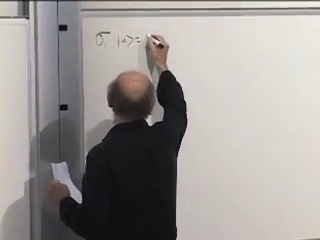
\includegraphics[width=0.62\linewidth]{lecture_05_figure_02.png}
\caption{Tabla completa de las acciones de Pauli que se utiliza en toda la comparación.}
\lectureframe{00:03:15}
\end{figure}

Ninguno de los espines constituyentes tiene una dirección preferente en ninguno de los dos estados:
\begin{equation}
  \expect{\sigma_i}_{\psi_\pm}=0,
  \qquad
  \expect{\tau_i}_{\psi_\pm}=0,
  \qquad i=1,2,3.
  \label{eq:l05-local-zero}
\end{equation}
Por ejemplo, el cálculo explícito solicitado para el estado con signo más da
\begin{align}
  \bra{\psi_+}\sigma_3\ket{\psi_+}
  &=
  \frac12
  \bigl(\bra{ud}+\bra{du}\bigr)
  \bigl(\ket{ud}-\ket{du}\bigr)\nonumber\\
  &=
  \frac12(1-1)=0.
  \label{eq:l05-sigma3-expectation}
\end{align}
Los términos cruzados se anulan porque \(\braket{ud}{du}=0\).

\begin{figure}[htbp]
\centering
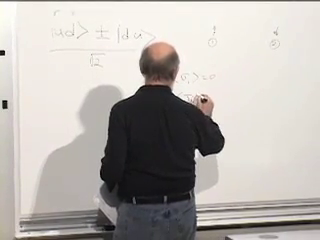
\includegraphics[width=0.78\linewidth]{lecture_05_figure_03.png}
\caption{El valor esperado para el estado con signo más se calcula aplicando \(\sigma_3\) y usando la ortogonalidad.}
\lectureframe{00:07:00}
\end{figure}

\begin{classroomqa}
\lecturetimestamp{00:07:13}
\audiencequestion{¿Significa un valor esperado nulo que una medición de un espín individual puede dar cero?}
\lecturerresponse{No. Una componente de un espín individual solo puede dar los resultados \(+1\) y \(-1\); \(\sigma_i\) no tiene ningún autovalor cero. La ecuación~\eqref{eq:l05-local-zero} dice que las mediciones repetidas equivalen al lanzamiento de una moneda equilibrada, no que un resultado individual sea cero.}
\end{classroomqa}

El primer diagnóstico plausible ha fallado. Los promedios locales no permiten distinguir el signo relativo, así que debemos medir una propiedad del par.

\section{El espín total identifica el singlete}

El momento magnético del par está representado por la suma vectorial
\begin{equation}
  \boldsymbol{\Sigma}
  =
  \boldsymbol{\sigma}+\boldsymbol{\tau}.
\end{equation}
Su componente tercera anula ambos vectores de la base:
\begin{align}
  (\sigma_3+\tau_3)\ket{ud}
  &=(1-1)\ket{ud}=0,\nonumber\\
  (\sigma_3+\tau_3)\ket{du}
  &=(-1+1)\ket{du}=0.
\end{align}
En consecuencia,
\begin{equation}
  (\sigma_3+\tau_3)\ket{\psi_\pm}=0.
\end{equation}
En cada ensayo, ambas elecciones de signo dan una componente tercera total nula.

La primera componente permite distinguirlos. A partir de la ecuación~\eqref{eq:l05-pauli-actions},
\begin{align}
  (\sigma_1+\tau_1)\ket{ud}
  &=\ket{dd}+\ket{uu},\nonumber\\
  (\sigma_1+\tau_1)\ket{du}
  &=\ket{uu}+\ket{dd}.
\end{align}
Por tanto,
\begin{align}
  (\sigma_1+\tau_1)\ket{\psi_+}
  &=
  \sqrt2\bigl(\ket{uu}+\ket{dd}\bigr),\nonumber\\
  (\sigma_1+\tau_1)\ket{\psi_-}
  &=0.
  \label{eq:l05-total-x}
\end{align}
El estado con signo más puede tener un valor esperado nulo para este observable, pero no es su autoestado de autovalor cero.

\begin{classroomqa}
\lecturetimestamp{00:13:02}
\audiencequestion{¿Qué resultados puede dar la componente total si el operador no anula el estado?}
\lecturerresponse{Cada espín individual da \(+1\) o \(-1\), así que la suma puede ser \(2\), \(0\) o \(-2\). Un valor esperado nulo no obliga a que el resultado sea cero en cada ensayo.}
\end{classroomqa}

La segunda componente completa la comprobación. Los factores de \(i\) se cancelan en la combinación antisimétrica:
\begin{equation}
  (\sigma_2+\tau_2)\ket{\psi_-}=0.
\end{equation}
Por tanto, las tres componentes anulan el estado con signo menos:
\begin{equation}
  \bigl(\boldsymbol{\sigma}+\boldsymbol{\tau}\bigr)
  \cdot\hat n\,\ket{\psi_-}=0
  \qquad\text{for every unit vector }\hat n.
  \label{eq:l05-singlet-any-axis}
\end{equation}

\begin{figure}[htbp]
\centering
\includegraphics[width=0.84\linewidth]{lecture_05_figure_06.png}
\caption{Cancelaciones componente a componente que identifican el estado con signo menos como un estado de espín total cero.}
\lectureframe{00:16:30}
\end{figure}

El estado antisimétrico \(\ket{\psi_-}\) es el \emph{singlete}. Es invariante bajo rotaciones: cualquiera que sea el eje, el espín total da el mismo resultado, cero. El estado simétrico de la ecuación~\eqref{eq:l05-two-signs} pertenece al sector triplete.

\begin{classroomqa}
\lecturetimestamp{00:19:06}
\audiencequestion{¿El resultado de espines opuestos se cumple solo en promedio?}
\lecturerresponse{En el singlete se cumple en cada ensayo. La ecuación~\eqref{eq:l05-singlet-any-axis} es una ecuación de autovectores, así que medir la misma componente en ambas partículas siempre da resultados cuya suma es el autovalor cero.}
\end{classroomqa}

\begin{classroomqa}
\lecturetimestamp{00:19:36}
\audiencequestion{¿Por qué el otro estado se llama triplete?}
\lecturerresponse{El nombre proviene de los tres estados del multiplete de espín total uno. Dejaremos su derivación para más adelante; para el cálculo actual basta distinguir el estado simétrico del sector singlete unidimensional.}
\end{classroomqa}

Si Bob mide cualquier componente de su electrón, sabe de inmediato qué resultado obtendría Alice al medir la misma componente en el suyo: el resultado de ella debe ser el opuesto. Esta es una correlación de Einstein--Podolsky--Rosen. Un par de monedas ocultas también puede llevar resultados opuestos, pero solo para una pregunta elegida de antemano. El singlete ofrece una anticorrelación perfecta para cualquier eje espacial que se elija.

\begin{classroomqa}
\lecturetimestamp{00:20:55}
\audiencequestion{¿Fueron Einstein, Podolsky y Rosen quienes descubrieron el entrelazamiento?}
\lecturerresponse{No. Schrödinger analizó el fenómeno e introdujo el término entrelazamiento. El argumento EPR planteó con especial claridad el problema de las correlaciones a distancia.}
\end{classroomqa}

\begin{classroomqa}
\lecturetimestamp{00:23:50}
\audiencequestion{¿La correlación inmediata viola la causalidad? ¿Importa qué observador mide primero?}
\lecturerresponse{No se transmite ningún mensaje utilizable. Los resultados locales de Alice siguen teniendo probabilidades iguales, mida Bob o no, en cualquier orden temporal inercial. Alice solo puede comprobar la correlación después de recibir el resultado de Bob por un canal clásico ordinario, que no puede superar la velocidad de la luz.}
\end{classroomqa}

\section{La desigualdad de Bell es un conteo clásico}

La importancia del resultado de Bell puede parecer cambiante. A veces parece el rasgo más profundo de la mecánica cuántica; otras, una consecuencia más inevitable del formalismo. Tanto Bell como Feynman podían adoptar ambas posturas. Sin embargo, la desigualdad es elemental. Lo sorprendente es que se viole.

Consideremos un conjunto ordinario de objetos. Cada objeto puede tener o no tener tres propiedades: \(A\), \(B\) y \(C\). Sea \(N(A,\neg B)\) el número de objetos que tienen \(A\) pero no \(B\). La lógica clásica de conjuntos implica
\begin{equation}
  N(A,\neg B)+N(B,\neg C)
  \geq
  N(A,\neg C).
  \label{eq:l05-bell-count}
\end{equation}
La demostración se basa en la inclusión de conjuntos
\begin{equation}
  A\cap C^{c}
  \subseteq
  (A\cap B^{c})\cup(B\cap C^{c}).
  \label{eq:l05-set-inclusion}
\end{equation}
En efecto, un elemento de \(A\cap C^c\) o bien pertenece a \(B\) o bien no pertenece a él. En el primer caso, pertenece a \(B\cap C^c\); en el segundo, pertenece a \(A\cap B^c\). Contar la unión solo puede sobrecontar el conjunto de la izquierda.

\begin{figure}[htbp]
\centering
\includegraphics[width=0.78\linewidth]{lecture_05_figure_07.png}
\caption{La demostración gráfica divide tres subconjuntos clásicos superpuestos en regiones no negativas.}
\lectureframe{00:31:15}
\end{figure}

De forma equivalente, asignemos a las regiones disjuntas del diagrama de tres conjuntos etiquetas de enteros no negativos \(N_i\). Ambos lados de la ecuación~\eqref{eq:l05-bell-count} incluyen las regiones que exige \(A\cap C^c\), pero el lado izquierdo incluye además otras regiones no negativas. No interviene aquí nada cuántico. Se trata de un teorema sobre subconjuntos y alternativas lógicas ordinarias.

\section{Convertir la afirmación sobre conjuntos en un experimento de espín}

Preparemos muchos pares de electrones independientes en el estado singlete y definamos tres proposiciones sobre el electrón 1:
\begin{align}
  A&:\ \text{spin 1 is up at }0^\circ\text{, along the third axis},\nonumber\\
  B&:\ \text{spin 1 is up at }45^\circ\text{ in the }zx\text{-plane},\nonumber\\
  C&:\ \text{spin 1 is up at }90^\circ\text{, along the first axis}.
  \label{eq:l05-abc}
\end{align}

\begin{figure}[htbp]
\centering
\includegraphics[width=0.82\linewidth]{lecture_05_figure_08.png}
\caption{Las tres proposiciones de espín se fijan en \(0^\circ\), \(45^\circ\) y \(90^\circ\) en un mismo plano.}
\lectureframe{00:39:00}
\end{figure}

En el singlete, la negación de una proposición sobre el electrón 1 puede expresarse como una proposición afirmativa sobre el electrón 2. Por ejemplo,
\begin{align}
  \neg B
  &:\ \text{spin 1 is down at }45^\circ\nonumber\\
  &\Longleftrightarrow
  \text{spin 2 is up at }45^\circ.
\end{align}
Del mismo modo, \(\neg C\) equivale a afirmar que el electrón 2 está orientado hacia arriba a \(90^\circ\).

\begin{classroomqa}
\lecturetimestamp{00:40:04}
\audiencequestion{¿Debe \(\neg C\) hacer que el electrón 2 esté orientado hacia abajo a \(90^\circ\)?}
\lecturerresponse{No. Primero negamos \(C\): el electrón 1 está orientado hacia abajo a \(90^\circ\). La anticorrelación perfecta del singlete implica entonces que el electrón 2 está orientado hacia arriba a lo largo de ese mismo eje. Hay que mantener separados los dos cambios de sentido.}
\end{classroomqa}

Para un conjunto grande, los conteos y las probabilidades solo difieren en el factor común correspondiente al número de pares preparados. La invariancia rotacional también implica que
\begin{equation}
  P(A,\neg B)=P(B,\neg C),
\end{equation}
porque el segundo experimento se obtiene al rotar el primero \(45^\circ\). Por tanto, la desigualdad clásica de Bell exigiría
\begin{equation}
  2P(A,\neg B)\geq P(A,\neg C).
  \label{eq:l05-bell-probability}
\end{equation}
Ahora necesitamos un método eficaz para calcular estas probabilidades.

\section{Las proposiciones se convierten en proyectores}

En un espacio vectorial tridimensional ordinario, un proyector elimina todas las componentes perpendiculares a un subespacio elegido. Un proyector unidimensional proyecta ortogonalmente un vector sobre una recta; uno bidimensional lo proyecta sobre un plano. Si \(P\) proyecta sobre un subespacio dado,
\begin{equation}
  P\ket{\alpha}=\ket{\alpha_P}.
\end{equation}

\begin{figure}[htbp]
\centering
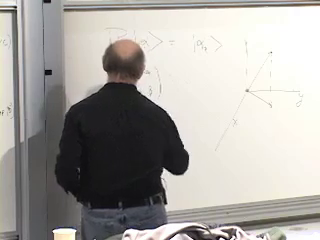
\includegraphics[width=0.76\linewidth]{lecture_05_figure_04.png}
\caption{La proyección geométrica y su notación mediante operadores se desarrollan en paralelo.}
\lectureframe{00:49:53}
\end{figure}

\begin{figure}[htbp]
\centering
\begin{tikzpicture}[scale=1.05,>=Latex]
  \draw[->] (-0.25,0)--(4.0,0);
  \draw[thick] (-0.25,-0.25)--(3.55,2.6);
  \draw[->,very thick] (0,0)--(2.25,3.05)
    node[above] {\(\ket{\alpha}\)};
  \coordinate (P) at (2.72,1.98);
  \draw[dashed] (2.25,3.05)--(P);
  \draw[->,very thick] (0,0)--(P)
    node[right] {\(\ket{\alpha_P}\)};
  \node[below right] at (3.1,2.25) {projected subspace};
\end{tikzpicture}
\caption{Una reconstrucción clara de la geometría de la proyección.}
\end{figure}

En el espacio de Hilbert de un espín, la proposición \(\sigma_3=+1\) corresponde al subespacio unidimensional generado por \(\ket{u}\). Su proyector actúa así:
\begin{equation}
  P_{\sigma_3=+1}
  \begin{pmatrix}\alpha\\\beta\end{pmatrix}
  =
  \begin{pmatrix}\alpha\\0\end{pmatrix},
  \qquad
  P_{\sigma_3=-1}
  \begin{pmatrix}\alpha\\\beta\end{pmatrix}
  =
  \begin{pmatrix}0\\\beta\end{pmatrix}.
  \label{eq:l05-projector-actions}
\end{equation}

\begin{classroomqa}
\lecturetimestamp{00:49:55}
\audiencequestion{¿El primer proyector indica hasta dónde llega el vector sobre un eje vertical?}
\lecturerresponse{No. Simplemente elimina el coeficiente ortogonal \(\beta\). Las componentes son amplitudes en el espacio de Hilbert, no coordenadas espaciales ordinarias del espín.}
\end{classroomqa}

\begin{figure}[htbp]
\centering
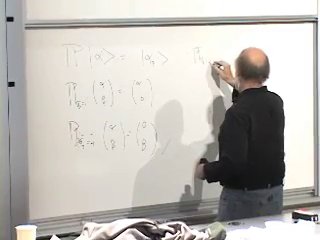
\includegraphics[width=0.78\linewidth]{lecture_05_figure_05.png}
\caption{Primero, los proyectores actúan sobre un espinor general; después, se expresan como matrices explícitas.}
\lectureframe{00:51:40}
\end{figure}

La forma matricial es
\begin{equation}
  P_{\sigma_3=+1}
  =
  \begin{pmatrix}1&0\\0&0\end{pmatrix}
  =
  \frac{I+\sigma_3}{2}.
  \label{eq:l05-p3}
\end{equation}
La misma construcción se aplica en cualquier dirección unitaria \(\hat n\):
\begin{equation}
  P_{\boldsymbol{\sigma}\cdot\hat n=+1}
  =
  \frac{I+\boldsymbol{\sigma}\cdot\hat n}{2}.
  \label{eq:l05-pn}
\end{equation}

\begin{classroomqa}
\lecturetimestamp{00:53:09}
\audiencequestion{¿Cuál es el proyector sobre \(\sigma_1=+1\)?}
\lecturerresponse{En la ecuación~\eqref{eq:l05-p3}, sustituye \(\sigma_3\) por \(\sigma_1\): \(P_{\sigma_1=+1}=(I+\sigma_1)/2\).}
\end{classroomqa}

La regla de Born adquiere ahora una forma útil para las proposiciones:
\begin{equation}
  P(\mathcal A\text{ is true in }\ket{\psi})
  =
  \bra{\psi}P_{\mathcal A}\ket{\psi}.
  \label{eq:l05-projector-born}
\end{equation}
Para un espinor normalizado \(\ket{\psi}=(\alpha,\beta)^T\), la ecuación~\eqref{eq:l05-projector-born} con \(P_{\sigma_3=+1}\) da \(|\alpha|^2\), como debe ser.

Este lenguaje pone de manifiesto la diferencia entre las proposiciones clásicas y las cuánticas. En la lógica clásica, una propiedad corresponde a un subconjunto de un conjunto. En mecánica cuántica, corresponde a un subespacio del espacio de Hilbert o, de forma equivalente, a su proyector. Las operaciones de retículo para subconjuntos y subespacios vectoriales no son las mismas; de esa diferencia surge la contradicción de Bell.

\subsection{El proyector conjunto de Bell}

Para \(A\wedge\neg B\), el electrón 1 debe estar orientado hacia arriba a lo largo del tercer eje y el electrón 2 debe estar orientado hacia arriba a lo largo de
\begin{equation}
  \hat n_{45}=\frac{\hat x+\hat z}{\sqrt2}.
\end{equation}
La componente pertinente del segundo espín es
\begin{equation}
  \boldsymbol{\tau}\cdot\hat n_{45}
  =
  \frac{\tau_1+\tau_3}{\sqrt2}.
\end{equation}
Por tanto, el proyector conjunto es
\begin{equation}
  P_{A\wedge\neg B}
  =
  \frac{I+\sigma_3}{2}
  \frac{I+(\tau_1+\tau_3)/\sqrt2}{2}.
  \label{eq:l05-joint-projector}
\end{equation}

\begin{classroomqa}
\lecturetimestamp{00:59:18}
\audiencequestion{¿Por qué aparece un factor \(1/\sqrt2\) en la componente de espín a \(45^\circ\)?}
\lecturerresponse{La dirección debe ser un vector unitario. Sus componentes en los ejes primero y tercero son ambas \(1/\sqrt2\), así que el observable correspondiente es \((\tau_1+\tau_3)/\sqrt2\).}
\end{classroomqa}

\begin{classroomqa}
\lecturetimestamp{01:00:52}
\audiencequestion{¿Está dividida entre dos toda la expresión \(I+\boldsymbol{\tau}\cdot\hat n_{45}\)?}
\lecturerresponse{Sí. El proyector es \(\bigl(I+\boldsymbol{\tau}\cdot\hat n_{45}\bigr)/2\); el factor \(1/2\) multiplica todo el numerador.}
\end{classroomqa}

Los dos factores de la ecuación~\eqref{eq:l05-joint-projector} actúan sobre factores tensoriales distintos y conmutan. Aplicarlos elimina primero todas las componentes en que el electrón 1 está orientado hacia abajo y, luego, todas las componentes restantes en que el electrón 2 está orientado hacia abajo a lo largo de \(\hat n_{45}\).

\section{Los números cuánticos invierten la desigualdad}

Sea
\begin{equation}
  \ket{\psi_s}
  =
  \frac{\ket{ud}-\ket{du}}{\sqrt2}
\end{equation}
el singlete. Empecemos con
\begin{equation}
  P(A,\neg B)
  =
  \bra{\psi_s}P_{A\wedge\neg B}\ket{\psi_s}.
\end{equation}
El factor \((I+\sigma_3)/2\) anula \(\ket{du}\) y deja \(\ket{ud}/\sqrt2\). El segundo factor da entonces
\begin{align}
  \frac{I+(\tau_1+\tau_3)/\sqrt2}{2}\ket{ud}
  &\notag\\[-0.3em]
  &=
  \frac12
  \left[
    \ket{ud}
    +\frac{\ket{uu}-\ket{ud}}{\sqrt2}
  \right]\nonumber\\
  &=
  \frac12
  \Biggl[
    \left(1-\frac1{\sqrt2}\right)\ket{ud}
  \nonumber\\
  &\qquad
    +\frac1{\sqrt2}\ket{uu}\Biggr].
  \label{eq:l05-projector-action}
\end{align}
El término \(\ket{uu}\) tiene solapamiento nulo con el bra singlete, y los factores de normalización restantes dan
\begin{equation}
  P(A,\neg B)
  =
  \frac14\left(1-\frac1{\sqrt2}\right).
  \label{eq:l05-pab}
\end{equation}

\begin{figure}[htbp]
\centering
\includegraphics[width=0.88\linewidth]{lecture_05_figure_09.png}
\caption{El cálculo con proyectores conserva el solapamiento de \(\ket{ud}\) y descarta la contribución ortogonal de \(\ket{uu}\).}
\lectureframe{01:08:20}
\end{figure}

La invariancia rotacional da el mismo resultado para el siguiente par de direcciones:
\begin{equation}
  P(B,\neg C)
  =
  \frac14\left(1-\frac1{\sqrt2}\right).
\end{equation}
Para \(A\wedge\neg C\), el segundo eje coincide con el primer eje espacial, así que
\begin{equation}
  P_{A\wedge\neg C}
  =
  \frac{I+\sigma_3}{2}\frac{I+\tau_1}{2}.
\end{equation}
El primer factor vuelve a dejar \(\ket{ud}/\sqrt2\). El término \(\tau_1\) produce \(\ket{uu}\), que es ortogonal al bra singlete, mientras que el término identidad sobrevive. Por tanto,
\begin{equation}
  P(A,\neg C)=\frac14.
  \label{eq:l05-pac}
\end{equation}
Al combinar los tres resultados,
\begin{equation}
  \underbrace{
  P(A,\neg B)+P(B,\neg C)
  }_{\frac12(1-1/\sqrt2)\approx0.146}
  <
  \underbrace{
  P(A,\neg C)
  }_{\frac14=0.25}.
  \label{eq:l05-bell-violation}
\end{equation}

\begin{figure}[htbp]
\centering
\includegraphics[width=0.84\linewidth]{lecture_05_figure_10.png}
\caption{El cálculo completo muestra que el miembro izquierdo de Bell es menor que el miembro derecho.}
\lectureframe{01:12:15}
\end{figure}

La ecuación~\eqref{eq:l05-bell-violation} invierte la ecuación~\eqref{eq:l05-bell-probability}. La conclusión no es que la mecánica cuántica se contradiga. Es que las correlaciones del singlete no pueden provenir de un modelo clásico local en el que las tres proposiciones sobre el espín tengan valores de verdad ordinarios, definidos según la teoría de conjuntos e independientes de la elección de medición a distancia. Una simulación clásica solo puede reproducir las correlaciones si abandona al menos una de las hipótesis de Bell, en particular la localidad.

\section{Qué pone a prueba el experimento de Bell}

La mecánica cuántica ya predice la violación. Además, el experimento debe cerrar la vía de escape clásica según la cual un detector informa al otro de qué configuración encontró o qué resultado obtuvo. Las dos estaciones deben estar suficientemente separadas, y las elecciones y detecciones deben producirse con tan poca diferencia de tiempo que una señal a la velocidad de la luz no pueda viajar entre ellas. El experimento de Aspect hizo convincentes, en la práctica, ese aislamiento y esa sincronización.

\begin{classroomqa}
\lecturetimestamp{01:13:15}
\audiencequestion{Si la mecánica cuántica ya da la respuesta, ¿nos enseñaron algo los experimentos de Bell?}
\lecturerresponse{Comprobaron si la naturaleza sigue la predicción cuántica en este experimento concreto de correlación y, aspecto crucial, hicieron independientes las dos estaciones de medición durante el tiempo pertinente para el recorrido de la luz. El control experimental y la sincronización fueron logros importantes por derecho propio.}
\end{classroomqa}

\begin{classroomqa}
\lecturetimestamp{01:18:19}
\audiencequestion{¿Qué aportó Bell después de que Einstein hablara de acción fantasmal?}
\lecturerresponse{Bell formuló una desigualdad cuantitativa. Identificó un experimento de correlación realizable cuya predicción cuántica descarta una explicación subyacente clásica y local, en vez de dejar la objeción en el plano del desasosiego filosófico. Bell mantuvo una postura ambivalente sobre si esto era inevitable o profundo y fue cuestionando cada vez más la mecánica cuántica estándar.}
\end{classroomqa}

Las partículas pueden estar separadas por kilómetros y seguir compartiendo un único estado conjunto, pero esto continúa siendo un experimento cuántico con sistemas pequeños. Las interacciones con el entorno tienden a destruir las relaciones de fase necesarias. Las moléculas de aire, los fotones parásitos y las perturbaciones térmicas pueden entrelazarse con el par; por eso, la separación debe realizarse en un entorno frío y bien aislado.

\begin{classroomqa}
\lecturetimestamp{01:19:53}
\audiencequestion{¿Que un estado común se extienda a gran distancia convierte esto en un objeto cuántico macroscópico?}
\lecturerresponse{Es más preciso describirlo como sistemas cuánticos pequeños y muy separados. La separación puede ser grande, pero preservar su función de onda conjunta se vuelve cada vez más delicado, porque las interacciones no controladas con el entorno destruyen la coherencia útil. Dos bolas de bolos ordinarias no permiten realizar el mismo experimento.}
\end{classroomqa}

\begin{classroomqa}
\lecturetimestamp{01:21:23}
\audiencequestion{¿Medir una partícula puede revelar información complementaria sobre la otra y permitir así eludir el principio de incertidumbre?}
\lecturerresponse{Se puede medir, por ejemplo, la posición de una partícula y el momento de la otra. Eso no equivale a medir simultáneamente observables que no conmutan en una misma partícula. No se ha eludido la restricción de incertidumbre para un sistema individual.}
\end{classroomqa}

\section{¿Cuándo significa «y» un producto?}

En el cálculo de Bell multiplicamos dos proyectores. Esto representa una conjunción solo cuando las proposiciones son compatibles.

\begin{classroomqa}
\lecturetimestamp{01:22:39}
\audiencequestion{¿Por qué el producto de dos proyectores representaba la conjunción lógica «y»?}
\lecturerresponse{Porque los dos proyectores conmutan. Uno actúa sobre el electrón 1 y el otro sobre el electrón 2, así que el orden es irrelevante y ambas propiedades pueden comprobarse a la vez. Para un solo electrón, \((I+\sigma_3)/2\) y \((I+\sigma_1)/2\) no conmutan; tener el espín orientado hacia arriba a lo largo de ambos ejes no es una proposición conjuntamente definida de este tipo.}
\end{classroomqa}

Este es otro aspecto en que las proposiciones cuánticas difieren de los subconjuntos ordinarios. La intersección clásica siempre existe. El análogo cuántico representado por un producto de proyectores solo tiene el significado lógico previsto cuando los subespacios pertinentes son compatibles.

Este mismo análisis apunta al problema de la medición. Un dispositivo de medición tiene un estado del indicador. Si un electrón con espín hacia arriba hace que el indicador se desplace en un sentido y uno con espín hacia abajo hace que se desplace en el otro, el electrón en superposición queda entrelazado con dos posiciones del indicador. Por tanto, la medición puede estudiarse como un entrelazamiento entre el sistema y el aparato. Dejaremos ese problema para más adelante y veremos un teorema más breve que solo requiere la linealidad.

\begin{classroomqa}
\lecturetimestamp{01:25:09}
\audiencequestion{¿Es útil considerar el colapso de la función de onda como una medición que determina el estado conjunto?}
\lecturerresponse{La pregunta forma parte del proceso de medición. El aparato y el sistema medido quedan entrelazados: un valor del espín se correlaciona con una posición del indicador y el otro valor con otra posición. Dejaremos para más adelante el análisis detallado de la medición.}
\end{classroomqa}

\section{La linealidad impide una fotocopiadora universal}

Solo necesitamos un hecho sobre la evolución temporal. Si un proceso físico transforma
\begin{equation}
  \ket{a}\longrightarrow\ket{a'},
  \qquad
  \ket{b}\longrightarrow\ket{b'},
\end{equation}
la linealidad exige que
\begin{equation}
  \alpha\ket{a}+\beta\ket{b}
  \longrightarrow
  \alpha\ket{a'}+\beta\ket{b'}.
  \label{eq:l05-linearity}
\end{equation}

Una fotocopiadora ordinaria puede reproducir información clásica con errores controlablemente pequeños. La exigencia cuántica es mayor: un mismo dispositivo debe duplicar todas las amplitudes de cualquier estado que se le presente. Por eso, a la imposibilidad de clonar también se la llama principio de imposibilidad de la fotocopiadora cuántica.

Imaginemos una máquina con un puerto de entrada y dos de salida. Si clona la base del tercer eje, debe realizar
\begin{equation}
  \ket{u}\longrightarrow\ket{uu},
  \qquad
  \ket{d}\longrightarrow\ket{dd}.
  \label{eq:l05-clone-basis}
\end{equation}
La máquina puede aportar energía, masa o carga a sus salidas; el obstáculo no está en llevar la cuenta de la conservación. La contradicción se refiere a la dependencia de la transformación respecto del estado.

\begin{figure}[H]
\centering
\includegraphics[width=0.86\linewidth]{lecture_05_figure_11.png}
\caption{Se exige que una máquina hipotética, con una entrada y dos salidas, duplique ambos estados de la base.}
\lectureframe{01:33:45}
\end{figure}

Ahora introduzcamos un espín orientado hacia la derecha:
\begin{equation}
  \ket{r}
  =
  \frac{\ket{u}+\ket{d}}{\sqrt2}.
  \label{eq:l05-right-state}
\end{equation}
Las ecuaciones~\eqref{eq:l05-linearity} y \eqref{eq:l05-clone-basis} obligan a que la salida sea
\begin{equation}
  \ket{r}
  \longrightarrow
  \frac{\ket{uu}+\ket{dd}}{\sqrt2}.
  \label{eq:l05-linear-output}
\end{equation}
Sin embargo, una clonación exacta exige dos copias independientes:
\begin{align}
  \ket{rr}
  &=
  \ket{r}\otimes\ket{r}\nonumber\\
  &=
  \frac12
  \left(
    \ket{uu}+\ket{ud}+\ket{du}+\ket{dd}
  \right).
  \label{eq:l05-cloned-output}
\end{align}
En la ecuación~\eqref{eq:l05-cloned-output} aparecen los términos mixtos que faltan en la ecuación~\eqref{eq:l05-linear-output}. Las dos salidas son distintas.

\begin{figure}[H]
\centering
\includegraphics[width=0.72\linewidth]{lecture_05_figure_12.png}
\caption{La linealidad solo produce los términos de espines paralelos, mientras que dos copias auténticas orientadas hacia la derecha contienen también los dos términos mixtos.}
\lectureframe{01:35:20}
\end{figure}

\begin{theorem}[No-cloning]
Ninguna máquina física puede clonar exactamente todos los estados cuánticos desconocidos.
\end{theorem}

\begin{proof}
Supongamos que una máquina clona los estados ortogonales de la base, como en la ecuación~\eqref{eq:l05-clone-basis}. La linealidad determina entonces su salida para la superposición, que es la dada en la ecuación~\eqref{eq:l05-linear-output}. Para clonar exactamente esa misma entrada se necesitaría la salida de la ecuación~\eqref{eq:l05-cloned-output}. Como los dos vectores de estado son distintos, la máquina universal supuesta no puede existir.
\end{proof}

La razón es estructural. Transformar \(\ket{\psi}\) en \(\ket{\psi}\otimes\ket{\psi}\) depende cuadráticamente de las amplitudes, mientras que toda evolución permitida del estado cuántico completo es lineal.

\begin{classroomqa}
\lecturetimestamp{01:35:49}
\audiencequestion{¿La demostración supone que las dos salidas son independientes?}
\lecturerresponse{Sí, porque dos clones deben ser copias independientes que puedan usarse por separado. Los sistemas independientes se combinan mediante el producto tensorial; por eso, dos copias orientadas hacia la derecha son \(\ket{r}\otimes\ket{r}\). Las salidas correlacionadas que no pueden usarse por separado no son dos clones.}
\end{classroomqa}

\begin{classroomqa}
\lecturetimestamp{01:37:20}
\audiencequestion{Un láser parece copiar el estado de un fotón mediante emisión estimulada. ¿Dónde falla el argumento?}
\lecturerresponse{El átomo y los modos electromagnéticos también intervienen. Su estado contribuye a la salida y, desde el punto de vista de la clonación universal, aparece como ruido. La clonación aproximada es posible, pero la clonación perfecta independiente del estado no lo es.}
\end{classroomqa}

\begin{classroomqa}
\lecturetimestamp{01:40:24}
\audiencequestion{¿Puede transferirse la información cuántica aunque no pueda duplicarse?}
\lecturerresponse{Sí. La transferencia es una operación distinta: no hace falta que el original conserve el estado. La imposibilidad de clonar prohíbe acabar con dos copias perfectas e independientes, no trasladar el estado de un portador a otro.}
\end{classroomqa}

\begin{classroomqa}
\lecturetimestamp{01:41:03}
\audiencequestion{¿Es necesario que el estado de entrada sea desconocido?}
\lecturerresponse{Si se conoce de antemano un estado, se pueden preparar más sistemas en ese mismo estado o construir un dispositivo adaptado a una base ortogonal elegida. Lo imposible es disponer de una sola máquina que acepte una entrada arbitraria y la duplique sin saber de antemano qué estado recibió.}
\end{classroomqa}

\begin{classroomqa}
\lecturetimestamp{01:42:35}
\audiencequestion{¿Cuál de las dos expresiones del estado orientado hacia la derecha es la salida real de la máquina?}
\lecturerresponse{La linealidad impone la ecuación~\eqref{eq:l05-linear-output}; clonar exige la ecuación~\eqref{eq:l05-cloned-output}. Su discrepancia es precisamente la contradicción.}
\end{classroomqa}

\begin{classroomqa}
\lecturetimestamp{01:43:40}
\audiencequestion{¿Se puede cuantificar la información adicional que contienen los estados entrelazados de dos partículas?}
\lecturerresponse{Un estado puro de un espín tiene dos parámetros físicos reales. Dos espines preparados por separado aportan cuatro, mientras que un estado puro general del espacio de Hilbert de dos espines, que es cuatridimensional, tiene seis una vez eliminadas la normalización y la fase global. Entre los estados adicionales hay estados entrelazados, cuyo grado de entrelazamiento puede cuantificarse mediante la entropía de entrelazamiento.}
\end{classroomqa}

\enlargethispage{4\baselineskip}
El signo de la ecuación~\eqref{eq:l05-two-signs} ha cumplido ya tres funciones. Ha seleccionado el único estado de espín total cero, ha proporcionado correlaciones que violan una desigualdad clásica de conjuntos y ha puesto de manifiesto la diferencia entre una evolución cuántica lineal y el acto no lineal de hacer dos copias. Cada resultado se deriva de tratar el estado conjunto como un vector en todo su espacio producto tensorial, en lugar de como una lista de propiedades locales preexistentes.
